\chapter{Abstraction}\label{C:abstraction}

% potential examples of abstraction?
% recipies
% programming?
% Programming in python is an abstraction. In reality the code we are writing gets translated into machine code...

\begin{displayquote}
 \textit{What is an abstraction?}
\end{displayquote}

A recipie is an abstraction. For example, pumpkin soup:

\begin{enumerate}
\tightlist
\item Boil stock (6 cups), garlic (1 clove), thyme (0.5 tsp) and pumpkin (4 cups) in a pot for 30 mins.
\item Puree the mixture.
\item Simmer for 30 minutes and then add cream (0.5 cups).
\end{enumerate}

This is an abstraction because it captures the essential details: from this recipe, you could make pumpkin soup.
While it ignores inessential details: the recipe doesn't tell you; where or what to cook in, where to get the
ingredients, which species of pumpkin to use, how to do the many actions needed to actually puree something, etc...
It also doesn't mandate; the time of day to perform this recipe, what clothes to wear (if any),
which music should be playing.

% Note that the essential / inessential details will depend on what you want to do with the abstraction.
% If we were bringing pumpkin soup to a friend, then the time of day would be important.

\vspace{5mm}

There exists a mathematical formalism, a  \href{https://en.wikipedia.org/wiki/Homomorphism}{homomorphism},
that allows us to more precisely reason about this transformation from
details to essence. Consider a ground space, $X$, (\textit{the reality of what
needs to be done. all the details}), and an abstract space $Y$ (\textit{our recipe}).
We are looking for a transformation between $X$ and $Y$ to preserves only the essential
structure in $X$. This can be written as $f: X\to Y$ such that;

% Another way to think about it, a 'structure preserving' map.

\begin{align*}
f(x \circ_G y) = f(x) \circ_A f(y)
\end{align*}

Where the $\circ$ is the preserved structure. \footnotemark[19]
A common example of a structure we might want to preserve is the order $\le$.
% In RL, we might want to preserve other operations such as the optimal policy or the Bellman operator.

\footnotetext[19]{Something that might not
be clear is that you need to be able to define $\circ$ on both $X$ and $Y$.
These definitions might be different from each other. For example on space might be continuious and the other discrete.}

In general, there are three steps to using abstraction to help solve a problem:

\begin{enumerate}
\tightlist
  \item Transform the problem to the 'abstract' domain. $f: X\to Y$
  \item Solve the problem $\mathcal S: Y \to Z$
  \item Lift the solution back to the original domain  $g:Z \to X$
\end{enumerate}

{\color{red}for example?!?}

\begin{displayquote}
 \textit{Why do we care?}
\end{displayquote}

The reasons we might care come back to wanting more efficient algorithms.
By throwing away inessential details, there is less to compute.
By throwing away unimportant factors, we have reduced the variance of our
observations and thus allow quicker learning.

% History.
%
% - Mathematics, category theory
% - Physics?
% - Comp sci, programming languages

\section{Abstractions for RL}

% homomorphisms dont segue into this very well...

% types of abstraction we will consider
There are a few different types of abstraction that can be considered for RL:
state abstractions \cite{Anand2019, Littman2006,Haarnoja,Cuccu2018,Zhonga,Vezzani2019,Abel2018,Duan2018,Abel2017,Silver2016a},
action abstractions \cite{Chandak2019,Bester2019,Tennenholtz2019,Nagabandi2019}, state-action abstractions \cite{Dayan1993,Barreto2017}, temporal abstractions \cite{Christodoulou2019, Rafati,Mankowitz2018,Harutyunyan2017,Fruit2017,Riemer2018,Bacon2018,Achiam2018,Pham2019,Konidaris2018,Haarnoja,Sutton1999,Fruit2017a,Bacon2016a,Jinnai2018,Nachum2018}.
These abstractions are often built for two goals; efficient exploration
(\href{https://en.wikipedia.org/wiki/Sample_complexity}{sample complexity})
and / or efficient optimisation (\href{https://en.wikipedia.org/wiki/Computational_complexity_theory}{computational complexity}).

\subsection{Classes of abstraction for RL}

% \begin{displayquote}
% \textit{But how might we contruct $Q^{\pi_{A}^* }$?}
% \end{displayquote}
%
% There are many different forms an abstraction might take, and ???

\begin{displayquote}
\textit{Given an abstraction, how might a learner use it?}
\end{displayquote}

The abstracted $Q$-function and policy might be constructed on spaces $X, Y$,
$Q_A: X \times Y \to \mathbb R$, $\pi_A: X \to \Delta(Y)$. We can now construct
different classes of learners by giving them access to different types of abstraction.

\begin{center}
  \begin{tabular}{ c || c | c | c | c }
    Abstraction & \textbf{X} & \textbf{Y} & \textbf{Value fn} & \textbf{Policy} \\ \hline \hline
    State & $\phi: S \to X$ & $A$ & $Q(\phi(s), a)$ & $\pi(a| \phi(s))$ \\ \hline
    Action & $S$ & $\psi: A \to Y$ & $Q(s, \psi(a))$ & $\pi(\psi^{-1}(y) | s)$\\ \hline
    State and action \footnotemark[5] & $\phi: S \to X$ & $\psi: A \to Y$ & $Q(\phi(s), \psi(a))$ & $\pi(\psi^{-1}(y) | \phi(s))$ \\ \hline
    State-action & \multicolumn{2}{c|}{$\varphi: S\times A \to X\times Y$} & $Q(\varphi(s, a))$ & $\mathop{\text{argmax}}_a Q(\varphi(s, a))$ \\ \hline
    Temporal (goal like) & $S$ & $f: S \to Y$ & $Q(s, f(s))$ &   \\ \hline
    Temporal (option like)\footnotemark[10] & $S$ & $g: \Omega \to Y$ & $Q(s, g(\omega))$ & $\pi(g^{-1}(y) | s)$ \\ \hline
  \end{tabular}
\end{center}

\footnotetext[5]{If the $Q$ fn is a linear function of the $\varphi(s, a)$ representation,
then this is known as the successor representation \cite{Dayan1993,Barreto2017}}

\footnotetext[10]{Goal like abstraction is actually a lot more general than is. But, it is easiest to understand when goals are picked to be states. Recent work has shown that goal-conditioned RL can work when you pick a certain return as the goal. This allows cool stuff - ref - ref.}

Where $\omega \in \Omega \subseteq A^k$.



\begin{displayquote}
\textit{Which class of abstraction should we use?}
\end{displayquote}

Possibly, the most interesting question is about the difference in performance between
the \textit{State and action abstraction} and the \textit{State-action abstraction}.
Or \textit{goal like} and \textit{option like} temporal abstractions.

\subsubsection{Examples}

\paragraph{State abstraction}

groups together states that are similar. For example, a 20 NZD note.
There are many different 20 NDZ notes that, for all actions, intents and purposes, are the same.
Someone may have written a note on the note, the note may have fold marks through it,
there might be different codes on the
bottom left corner or right hand side, it might be an older version, ....

Rather than describing these inessential details, we can abstract away from them.

\begin{figure}[h!]
\centering
\includegraphics[width=0.7\textwidth,height=0.2\textheight]{../../pictures/images/nz20.png}
\caption{A 20 NZD note.}
\end{figure}

\begin{figure}[h!]
\centering
\includegraphics[width=0.7\textwidth,height=0.2\textheight]{../../pictures/drawings/my-nz20.png}
\caption{An artist's abstract rendering.}
\end{figure}

\paragraph{Action abstraction}

groups together actions that are similar. For
example, both action $i$ and action $j$ might yield the same rewards and change in state,
in which case, we can just relabel them as the same action.

\begin{figure}[h!]
\centering
\includegraphics[width=0.8\textwidth,height=0.2\textheight]{../../pictures/drawings/hungry-caterpillar.png}
\caption{Consider a hungry caterpillar. It wants to move towards the leaf. But this is a complicated task! Move your 3rd leg up, your 7th leg down, 11th leg slightly forward, etc...}
\end{figure}


\begin{figure}[h!]
\centering
\includegraphics[width=0.8\textwidth,height=0.2\textheight]{../../pictures/drawings/full-caterpillar.png}
\caption{But, what if the caterpillar could specify actions in another way?
Rather than specifying leg movements, it could pick a direction to move,
which would specify the movement of multiple legs.}
\end{figure}

\paragraph{State-action abstraction}

Groups together state-actions that achieve similar results. This class of abstraction
should be more powerful than state and action abstraction. Consider a mirror symmetric maze.

\begin{figure}[h!]
\centering
\includegraphics[width=0.8\textwidth,height=0.4\textheight]{../../pictures/drawings/maze.png}
\caption{A symmetric maze, the goal(s) are shown in red.
Consider two different, but 'similar' positions, shown in blue and green.}
\end{figure}

Given this setting, we can construct a representation of the state \footnotemark[11] where,
we have $Q^{\pi}(s, a) = Q^{-\pi}(-_xs, -a), \forall \pi$.
Where the negative operator $-_x$ only effects the horizontal ($x$) axis $s = (x, y), -_xs = (-x, y)$.
And $-\pi := \pi(-a|-_xs)$.

\footnotetext[11]{To construct this representation, we set the state to be centered around the mirror plane.
So the blue player is at location $(-3, 9)$ and the green player is at location
$(3, 9)$. And we equip the players with the actions $(+1, 0), (-1, 0), (0, -1), (, +1)$ (aka; up, down, left, right).}

State abstraction would not be able to group together the blue and green positions.
As moving left from blue is not equivalent to moving left from green.

\paragraph{Temporal abstraction}

We can group together goals / options that achieve 'similar' results.
For example, the pumpkin recipe above: for the many ways there are to boil broth
(in pot, in a jug, over a wood fire, in the oven, ...), group them together.
For the many ways to puree some pumpkin (with a rolling pin and some vigor, with a blender, ...), group them together.

The intuition behind both goal-like and option-like temporal abstractions is that
we can decompose a sequential decision problem into a set of shorter, easier to solve, parts.

\subsection{Discovery}

\begin{displayquote}
  \textit{Where do abstractions come from?}
\end{displayquote}

In the earlier sections we considered how an agent might use a given abstraction.
But where did that abstraction come from? Did someone construct it for the given task?
Or can abstractions be discovered automatically?

To build an abstraction, you need some notion of how two objects can be similar. (ref?!)
% (need a ref for this?!)
This allows you to group the 'similar' objects together, thus building an abstraction.
In RL there are many possible notions of similarity. But which ones are sensible?
And which ones allow us to efficiently finding the optimal policy?

\vspace{5mm}

For example, state abstraction: Li et al. \cite{Littman2006} give five classes of
state abstraction in which they group states based on various similarities \footnotemark[20];
\footnotetext[20]{Similarity and preservation are dual notions.
Similarity tells us which objects we can group together,
preservation tells us which objects we cannot group together.}

\textit{intuitively,
$\phi_{\text{model}}$ preserves the one step model,
$\phi_{Q_{\pi}}$ preserves the state-action value function for all policies,
$\phi_{Q^{* }}$ preserves the optimal state-action value,
$\phi_a^{* }$ preserves the optimal action and its value,
$\phi_{\pi^{* }}$ preserves the optimal action.}

{\color{red}haven't mentioned what these abstractions are being used for?!?}
i.e. constructing a new MDP with $\{\tilde S, A, \tilde P, \tilde r, \gamma\}$

In general, there seem to be a few different dimensions to designing similarity measures for RL.

\begin{itemize}
  \tightlist
  \item What objects do we want to base our similarity measure on? States, actions and / or rewards, or some combination or representation of them,
  \item How will we characterise these objects? By considering n-step futures, their expected value versus a rollout \footnotemark[9],
  \item Should these similarities hold for all policies or just a subset (such as just the optimal policy)? (OR?!?)
\end{itemize}

\footnotetext[9]{These can be unified using the $Q(\sigma)$ algorithm \cite{Asis2018}}

{\color{red}How does on/off policy come into this!? Is this family complete?!}

More formally. Let $X \in {S, A, R}^{* }$. $P \subset \Pi$

\begin{align*}
c(x) = \mathop{\mathbb E}_{\hat x \sim E(x, \pi)} [\gamma^t \hat x(t)] \\
\chi(x, x'; \gamma) = \int_{\pi \in \mathcal P} D(c(x, \pi, \gamma), c(x, \pi, \gamma))
\end{align*}

{\color{red}Work in progress...}

It would be nice to show that all abstractions of interest live in this happy family. (!!)

\vspace{5mm}

\begin{displayquote}
	\textit{How might we infer that two objects are similar?}
\end{displayquote}

There are two possibilities: we can infer that two objects are similar because we have seen it,
we have data / evidence / experience of the form $f(x_i) = f(x_j)$.
Alternatively, we can infer that two objects are similar because we have found a pattern.
For example, we might have seen that rotations of $45, 90, 135, 180$, are all similar, therefore our first guess
is that rotations of $225, 270, 315$ are also similar. (priors / inductive bias / generalisation)
This insight motivates our work on symmetric abstractions \ref{symmstric-abstractions}.
Which give the ability to generalise knowledge about a similarity to other similarities.


\subsection{Evaluating abstractions}

\begin{displayquote}
\textit{But which type of abstraction should we pick?}
\end{displayquote}

Ideally we would pick the most coarse abstraction, as a coarse abstraction means we have grouped together many objects. (ref)
Thus it has potential for the greatest increases in computational and sample efficiency.
But. Coarseness is not the only property of an abstraction we care about.
It must also allow you to represent near optimal policies and it must allow you
to efficiently find those near optimal policies.

% Need to be able to easily evaluate them.

\subsubsection{Coarse abstractions}

Coarse (as opposed to fine) is a term from topology.
A (more) coarse abstraction describes an abstraction that has a looser notion of similarity.
Thus more things are considered similar.
(Coarseness captures looser concepts such as a 'high level' abstraction or a 'general' abstraction).

\textit{We say $\phi_1$ is finer (less coarse) than $\phi_2$, denoted $\phi_1 \ge \phi_2$,
iff for any states $s_1, s_2 \in S, \phi_1(s_1) = \phi_1(s_2)$ implies $\phi_2(s_1) = \phi_2(s_2)$.} \ref{Littman2006}

Anytime $s_1$ and $s_2$ are considered similar in an abstraction, then a coarser
abstraction will also consider them to be similar, and there might also be other similar states.

So the most coarse abstraction would be where everything is mapped to the same abstract state.
$\forall s_i, s_j\in S: \phi(s_i)=\phi(s_j)$.

% The comparison of topologies constructed using varios k length optiions.
% With increaseing k, the topology of the abstraction is always coarser??

\begin{displayquote}
\textit{Why are coarse abstractions desirable?}
\end{displayquote}

By throwing away inessential details;
\begin{enumerate}
  \tightlist
  \item we have reduced the variance of our observations and thus allow quicker learning.
%  \item we have implicitly included an inductive bias towards 'simple' MDPs. (generalisation!) No.
  \item we will not waste time exploring them.
  \item there is less to compute.
\end{enumerate}


% In this case, fewer states. Since complexity of solving MDPs is $\mathcal O(|S| ???)$, this is great.

{\color{red}TODO Want formal version of 1-3!!!}

% reduce variance in estimates   \cite{Allen-Zhu2016a,Johnson2013a}
  % take size of smallest partition to be X. use this to say: reduces variances by at least a factor of X.
% spend less time exploring unimportant states / actions
  % in the ?? abstraction case.
% less states / actions to attempt to design a control for

\subsubsection{Near optimal abstractions}

%  but. how can we analyse them?
% tools we can use to analyse an abstraction
Imagine we have a state abstraction, a road is a road, there is no real difference
between them; gravel, winding, motorway, cliffs-on-either-side...
One of the first things we want to know about the abstraction is:
is it possible for me to act optimally
using this abstraction? If not, what's the damage? In this case, does driving 100kph on every road --
because they are all pretty-much-the-same -- lead to suboptimal results? Probably.
More precisely, we want know to whether the optimal policy can be approximately represented within an abstracted MDP.

% formal
This notion of sub-optimality can be formalised as the representation error of the optimal
policy. \cite{Abel2017} Given an abstraction, we want to know how well the abstraction can represent the optimal policy.

\begin{align}
\forall_{s\in S} \mid V^{\pi^* }(s) - V^{\pi_{A}^* }(s) \mid \le \epsilon
\end{align}

Where $\pi^{* }$ is the optimal policy, and $\pi_{A}^{* }$ is the lifted optimal
policy found using the abstraction.

This notion can be generalised to other types of abstraction, for example
Nachum et al. 2018 \cite{Nachum2018} extend this concept of near optimal
representation of the optimal policy to goal-like temporal abstraction. \footnotemark[13]

\footnotetext[13]{To do this, Nachum et al. 2018 \cite{Nachum2018} quantify
how many of the possible low level behaviours can be produced by different choices of goal.
This is roughly a measure of the invertability of the 'low level' policy from
state-goals to temporally extended actions.
This allows them to reason about which behaviours are representable using goals,
and thus whether a 'high level' policy choosing these goals can approximate the optimal policy.}

\subsubsection{Efficiently solvable abstractions}

Just because a near optimal policy exists (under our abstraction), that does not mean it will be easy to find.
We might require large amounts of data or computation.


\paragraph{Efficient exploration}
% What is needed for efficient exploration. And when is 'it' preserved? !!!

For $Q$-learning, Jin el at. \cite{Bubeck2018} show that efficient exploration ($\mathcal O(\sqrt{H^3SAT})$\footnotemark[13]) can be
achieved with a UCB-Bernstein type exploration bonus, compared to the inefficient exploration ($\mathcal O(\sqrt{H^4SAT})$),
achieved by the UCB-Hoeffding type exploration bonus. To achieve this, the UCB-Bernstein type exploration bonus needed to incorporate an
estimate the variance of the values, while the Hoeffding exploration bonus relied only on visitation counts.

\footnotetext[13]{$\mathcal O(\sqrt{H^3SAT})$ tells us that the expected regret scales, in the worst case, as a function of $\sqrt{H^3SAT}$.
Where $H$ is the planning horizon, S is the size of the state space, $A$ is the size of the action space and $T=KH$, where $K$ is the total number of episodes played.}

This tells us that, if we want to preserve our ability to efficiently explore (in the above sense) we need to preserve the value for all policies.
Because ....
If the value under the abstraction of even a single state is wrong, it could arbitrarily change the variance estimates
(well, that isnt true...?!? depends on the value of the other states we might share with)

Is this true in general, or specific to Q-learning with exploration bonuses? Future work.

\paragraph{Efficient control}

% this is about preserving the bellman eqn.
Fortunately, if we have preserved the state-action values, we have preserved the Bellman equation and can use it to guide the search. {\color{red}(ref / proof!!)}

\begin{align*}
\Delta Q(s, a) &= \alpha \big(T(Q)(s, a) - Q(s, a) \big) \\
T(Q)(s, a) &= r(s, a) + \gamma \mathop{\mathbb E}_{s'\sim \tau(\cdot|s, a)} \mathop{\mathbb E}_{a'\sim \pi(\cdot|s)} Q(s', a') \tag{SARSA} \\
T(Q)(s, a) &= r(s, a) + \gamma \mathop{\mathbb E}_{s'\sim \tau(\cdot|s, a)} \mathop{\text{max}}_{a'} Q(s', a') \tag{Q-learning}
\end{align*}

We can see that if the optimal policy's state-action value, $Q^{* }(s, a)$, is preserved, then ...???

\paragraph{Efficient inference}
% What is needed for efficient inference (in RL). And when is 'it' preserved? !!!

What are we inferring? Values, models, ???

% Efficient inference and RL dont really go together...!?

\cite{Allen-Zhu2016a}
% these refs actually show faster convergence not faster learning!?



\begin{center}\rule{0.5\linewidth}{\linethickness}\end{center}
  {\color{red}Are these properties necessary and / or sufficient for good performance of an abstraction?}
  % we are missing tools an analyse the methods of discovery
  % methods of discovery = !?!?
\begin{center}\rule{0.5\linewidth}{\linethickness}\end{center}

So, now that we have a notion of better / worse abstractions. Let's consider the abstractions
that Li et al. \cite{Littman2006} defined.

Li et al. \cite{Littman2006} show that $\phi_G \le \phi_{\text{model}} \le \phi_{Q_{\pi}} \le \phi_{Q^{* }} \le \phi_a^{* } \le \phi_{\pi^{* }}$

So we should prefer $\phi_{\pi^{* }}$? But. There exist examples where the
optimal policy found using $\phi_{\pi^{* }}$ is not optimal in the ground MDP \cite{Jong2005}.
% above. which of the three issues i outlined above does this fall into?!

Then our next preference is $\phi_a^{* }$. But. When using $\phi_a^{* }$ the value of non-optimal actions has not been preserved,
therefore we cannot use the Bellman operator to guide optimisation. ({\color{red}TODO} see experiments / proof in ref).

Again, our next preference is $\phi_{Q^{* }}$ .
But. $\phi_{Q^{* }}$ has not preserved the state-action values for all policies,
therefore we cannot use on policy learning ({\color{red}TODO} see experiments / proof in ref).


% TODO
% If two states have the same value under all possible policies, does this mean
% they have the same rewards and transition probabilities?!?

% $V(s) - V(s')$ as a similarity measure tells us very little. Because...? Many collsions?! But if over all policies then is ok!?
% Why doesnt this simple baseline work. Try it out?! Explain.
% On a simple MDP, on atari. How to implement? Need to learn $\chi(s, s')$.
% It will learn whether two state are similar under many different policys. As we train it...
% For every state in our replay buffer, is the return similar to other states?
% Just sample a minibatch and compare those states.
% Does this allow us to build more general abstractions?

\subsubsection{Complexity of finding an abstraction}

We hope to build learners capable of discovering an abstraction to help them efficiently solve the problems they are given.
But, the efficiency gains of using an abstraction \underline{must} offset the cost of
discovering that abstraction! Else, why did we bother...?

\begin{displayquote}
\textit{The challenge in the single-task case is overcoming the additional cost of discovering [an abstraction];
this results in a narrow opportunity for performance improvements, but a well-defined objective.
In the ... transfer case, the key challenge is predicting the usefulness of a particular [abstraction] to future tasks, given limited data.}\cite{Konidaris2019}
\end{displayquote}

{\color{red}TODO}

\paragraph{Single task case}

For example, in model-based RL. The agent attempts to learn (/ discover) the
transition and reward functions. Once discovered, they can be used to find the optimal policy, without requiring data!
But, to learn the transition and reward function, a lot of data might have been needed.

In this case, the cost of discovery, the cost to learn the transition functions can be offset
by the ability for the agent to easily generalise to new tasks (aka new reward functions).
As it does not need to relearn the transition function.

But, there do exist learning problems where the transition function has many
factors of variance, while the value can be easily predicted from observations.
Thus ...
{\color{red}not the best example for talking about abstraction!?}

\paragraph{Transfer case}

Without biases, there is no hope in general. The no free lunch theorem.
As often as we guess right about the "usefulness of a particular [abstraction] to future tasks",
there will be another set of future tasks where we are wrong.

An abstraction (say hierarchical) is not always the answer. There are problems in which
hierarchies do worse than ???. ref.

\begin{center}\rule{0.5\linewidth}{\linethickness}\end{center}

To evaluate an abstraction for the single task case, we need to analyse the
complexity of all three steps (abstract, solve, lift), and compare them against
solvers that do not abstract.

In the tansfer case, we need to construct a set of task. And count the
complexity of discovering the abstraction, and then the cost of solving
and lifting it for each new task.

\subsection{Related work: Representation learning for RL}

% \begin{displayquote}
%   \textit{[Abstraction] is a mapping from one problem representation to a new representation, while preserving some properties} (Littman / Walsh.)
% \end{displayquote}

{\color{red}There is a lot to talk about here...}

Representations that attempt to preserve
\begin{itemize}
\tightlist
  \item the mutual information between ? and ??.
  \item knowledge required to predict the next state
  \item ... geometric bellamere
  \item \cite{Nachum2018}
  \item autoencoders...
  \item next step prediction.
\end{itemize}

But with what guarantees?
